\documentclass[a4paper]{sbgames}               % final
%\usepackage[scaled=.92]{helvet}
\usepackage{times}
\usepackage{graphicx}

%% use this for zero \parindent and non-zero \parskip, intelligently.
\usepackage{parskip}

%% the 'caption' package provides a nicer-looking replacement
\usepackage[labelfont=bf,textfont=it]{caption}

\usepackage{url}

%% Paper title.
\title{FPS: First ``Paper''  Shooting}

%% Author and Affiliation (multiple authors). Use: and between authors

\author{Name1 A. Surname1\\ Digital Games Lab 
        \and Name2 B. Surname2\\ Name3 C. Surname3\\ ZZZZ University
        \and Name4 D. Surname4\\ Farwest Research Center 
}
\contactinfo{\{name1,name3\}@xxx.yyyy.yyy \\
             *name2@zzzz.vvvv.vvv
}
%% Keywords that describe your work.
\keywords{Real-time Strategy, Relief Mapping, Shortest Path Algorithm, First Person Shooting}

%% Start of the paper
% Attention: As you need to insert EPS images in Postscript, 
% you need to insert PDF images into PDFs. 
% In the text, extensions cancbe omitted (latex use .eps, pdflatex get .pdf) 
% To convert them: epstopdf myimage.eps
\begin{document}

\teaser{
  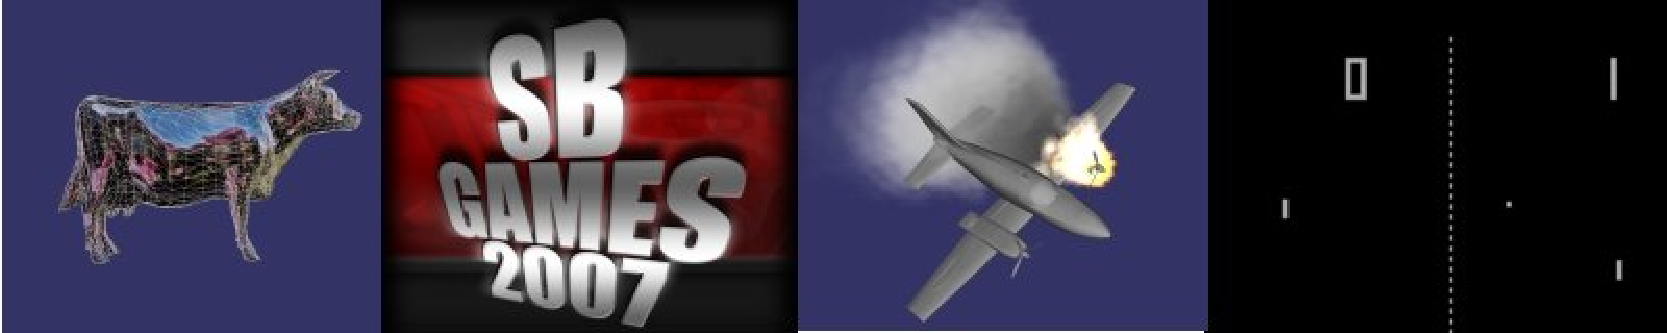
\includegraphics[width=\linewidth]{sample.pdf}
  \caption{Optional image}
}

%% The ``\maketitle'' command must be the first command after the
%% ``\begin{document}'' command. It prepares and prints the title block.

\maketitle

%% Abstract section.

\begin{abstract}

  This meta-paper describes the model to be used in papers and posters
  for SBGames. In the subsection Author's contact, make reference to
  the same symbol used in the affiliation.
\end{abstract}

%% The ``\keywordlist'' command prints out the keywords.
\keywordlist
\contactlist

\section{Introduction}

The document specifications are: paper size A4; margins: Top = 2.0 cm,
Bottom = 2.5 cm, Left = 2.5 cm, Right = 2.0 cm; 2 columns with Width =
7.85 cm and Spacing = 0.8 cm. You should not number the pages.

The typeface reference of your paper/poster is 10 point Times New
Roman, single line spacing, justified. The exceptions are:

\begin{itemize}

\item Title (see above)
\item Affiliation: 12 point Times New Roman, centered
\item Internet addresses and computer codes: 9 point Courier New
\item Caption (Figures and Tables): 9 point Times New Roman, centered under figure or table.
\item Section Head: 12 point Arial, bold, left aligned, numbered
\item Subsection Head: 10 point Arial, bold, left aligned, numbered
\item References: 9 point Times New Roman
\end{itemize}


\section{Related Work}
\label{sec:related-work}
It is strongly recommended that your paper has a section named Related
Work. This is a tradition in the most important international
conferences.


\section{General Recommendations}
\label{sec:gener-recomm}

Avoid to leave a section or subsection head isolated in the previous
column or page.

Only the first paragraph of a section starts with no tab; any other
paragraph starts with a tab of 0.5 cm. Every paragraph and head has a
blank line before them. You should avoid writing a subsection
immediately after a section head; trying to have at least a sentence
explaining the section.


\subsection{Citations and References}

SBGames citation format is the familiar ???author year??? format (quite
similar to the one used by the SIGGRAPH conferences), also called
Harvard notation. Although the Harvard notation uses parentheses,
SBGames citation format uses brackets. Detailed information about the
Harvard notation can be found elsewhere~\cite{Holland:2006:CRH}.

The Harvard notation can be summarized as follows. The year is
separated from the author by a single space. If the article has two
authors, their last names are used, separated by the word \emph{and}. If
the article has three or more authors, the primary authorss name,
followed by et al. are used. Multiple citations are separated by
semicolons:~\cite{Park:2006:DSI,kartch:2000:ERA}.

The reference list must be unnumbered, alphabetized by primary
author last name, with the author list set in small caps, followed
by the year of publication, followed by other information. The page
number, if any, appears last in the reference. The second and
successive lines of each entry are indented 0.5cm. Journal, book,
thesis, and conference proceeding titles are set in italic type. See
examples in the section References below. File \emph{sbgames.bst}
refereced below, perform automatic bibliography formatting.


\subsection{Figures, Images, and Tables}
\label{sec:figur-imag-tabl}

You may have figures crossing the columns. However, large images
should be placed at the very end of the paper or poster. You should
avoid framing the figure with a visible line (unless the border is
part of the figure). Figure~\ref{fig:example} illustrates this situation.  

\begin{figure} 
  \centering 
  
\includegraphics[width=0.8\linewidth]{example.pdf}
 \caption{Example of image} 
 \label{fig:example} 
\end{figure}


In order to know if an image has sufficient resolution to be
faithfully reproduced, you should multiply the size in cm by the
factor 120. For example, an image of 5 cm x 7.5 cm in your document
should have a resolution of no less than 600 pixels x 900 pixels.
Another example: a screenshot of your entire 1024 x 768 display
monitor should be no larger than 8.5 cm x 6.4 cm when positioned in
your document.

Table titles should be centered above the tables.

As specified in CFP, papers must be in PDF format. So, the best way to
generate PDF from .tex is using \emph{pdflatex} (Unix), directly.
Then, figures include into the text must be in PDF format. EPS format
is employed, when latex, and dvips are adopted. But, using these
programs, a ps-to-pdf conversion is required and can introduce quality
loss. Please: use \emph{pdflatex} to achieve high quality.
 

\section{Generating the paper in PDF file format}
\label{sec:generating-pdf-file}

Use \emph{template.tex} and  \emph{template.tex} to write your paper and enumerate bibliographic references. So, run:

\begin{description}
\item pdflatex template
\item bibtex template
\item pdflatex template
\item pdflatex template
\end{description}

That's it. You can rename template.tex and .bib. So, keep
\emph{sbgames.cls} and \emph{sbgames.bst} without modifications. They
are required to format text and bibliography according to SBGAMES
format.


\section{How to submit}
\label{sec:how-submit}

Each manuscript must be submitted electronically using the JEMS
submission site at \url{https://submissoes.sbc.org.br/sbgames2007} ONLY PDF
file format is accepted. An additional 10 MB will be available for the
(optional) ZIP file with the supplementary material.

Every co-author of a manuscript must also be registered as a user of
JEMS before the manuscript is submitted. Instructions on how to
register new JEMS users and how to retrieve forgotten JEMS passwords
are available at the same URL above. PLEASE MAKE SURE THAT EVERY
CO-AUTHOR IS INCLUDED AT THE TIME OF SUBMISSION. WE CANNOT LATER ON
ADD AND/OR REMOVE AUTHORS FROM SUBMITTED PAPERS.

Upon logging on at \url{https://submissoes.sbc.org.br/sbgames2007}
select the icon ``submit paper'' for the track ``Computing - Full
Papers'', in order to submit a full paper. You will then be taken to a
page with the title "Submit a paper to SBGAMES 2007 - Computing
Track". Fill in the paper registration information requested in that
page (don't forget to chose the keywords for your paper at the bottom
of the page) and then click on the ``submit'' icon, in order to
complete your paper's registration. After doing so, you will view a
page called "Registering Paper". The first line after the title of
this page should say ``Paper $<$5digits$>$ created'', where
$<$5digits$>$ is a five-digit number assigned by JEMS to your
manuscript. Before you upload your manuscript, include this five-digit
number in the place where you would normally put the author names (for
instance, by including the command
$\backslash$\emph{author}\{Manuscript number $<$5digits$>$\} in your
LaTeX source file).

After you have generated the final PDF file containing the manuscript
number (which should be renamed as $<$5digits$>$.pdf), you can upload
it immediately by following the "upload" link available on the page
"Registering Paper", or log out of the JEMS site and return later to
upload your paper.  If you choose the latter option, an "Upload" icon
for each registered manuscript will be accessible from your SBGAMES
2007 home page within JEMS. In any case, please upload the PDF file
with your manuscript first and then, if desired, return to the
manuscript upload page (either using your browser's "Back" button or
through your SBGAMES 2007 JEMS home) and upload the optional ZIP file
with the supplementary material.  You should receive an e-mail
confirmation every time you perform an upload.

\section{Conclusion}
\label{sec:conclusion}

The final sections of your work are: acknowledgements and references.
These final sections are not numbered.

\section*{Acknowledgements}

To Robert, for all the bagels.

\bibliographystyle{sbgames}
\bibliography{template}
\end{document}